\section{Part: GPS }\label{sec:q3}    

\subsection
I give more than required 6 for the sake of the benefit of us all (but in the exam it is important to put the exact number asked).
\begin{enumerate}
	\item Integer ambiguity
	\item Atmospheric errors
	\item Clock errors
	\item Doppler effects
	\item Ephemeris error of GNSS satellite
	\item Relativistic error
	\item Multipath
	\item Receiver noise
\end{enumerate}
	
\subsection{}
Applying double differencing mitigates the following errors:
\begin{enumerate}
	\item Atmospheric errors
	\item Clock errors
	\item Ephemeris error of GNSS satellite
\end{enumerate}



\subsection{}
There are 6 possible double differences. For this procedure 2 ground stations are needed (we have two, therefore no possible variations of the configurations) and 2 satellites - we have 4 at our disposal, which gives us 6 different possible pairs of satellites.

\subsection{}
Dilution of precision is a parameter describing quantitatively, how large would be the error caused by geometrical distribution of the satellites on the sky. In other words, the greater the PDOP, the less reliable the position estimation. It can be illustrated by the figure below. Satellites located close to each other in the sky would give large possible area of location, whereas ranges from distanced satellites (in terms of the sky seen by the observer) would give more precise location due to bigger angle between the two radii led from the satellites to the observer.

\begin{figure}[H]
		\centering
		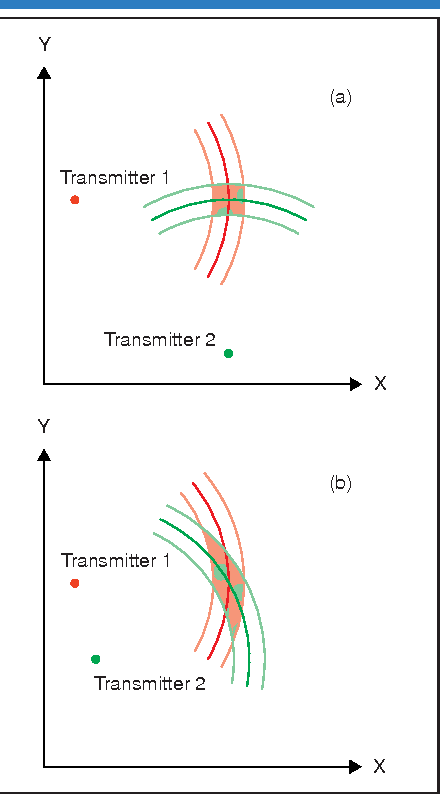
\includegraphics[width=0.6\linewidth]{pdop.png}
		\caption*{Source:Semantic Scholar}
\end{figure}


\subsection{}
Elevation mask is a technique of ignoring signal from satellite that are low above the horizon (mask might be applied e.g. for elevation of 10 degrees, meaning that all satellites that at the moment of signal emission are below this value of elevation in the local horizon reference frame of the observer would be ignored). This technique serves the purpose of avoiding high atmospheric errors (larger travel paths through the atmosphere result in higher errors). However, selecting only satellites higher up in the sky results in greater value of PDOP (undesirable). Balancing between those two is a tradeoff the designers of navigation systems need to face.
	
